\subsection{Nhận diện tư thế người}
% Slide 1: Section Overview
\begin{frame}{Nhận diện Tư thế Người và Phát hiện Té ngã}
    \begin{block}{Tổng quan}
        Hệ thống tích hợp nhận diện tư thế (MediaPipe Pose) và phát hiện té ngã dựa trên đặc trưng động học/tư thế.
        \begin{itemize}
            \item Ứng dụng: Giám sát an toàn, phát hiện té ngã.
            \item Nền tảng: Thị giác máy tính thời gian thực.
        \end{itemize}
    \end{block}
\end{frame}

% Slide 2: Nhận diện Tư thế Người
\begin{frame}{Nhận diện Tư thế Người}
\begin{columns}[T]
    \begin{column}{0.45\textwidth}
        \centering
        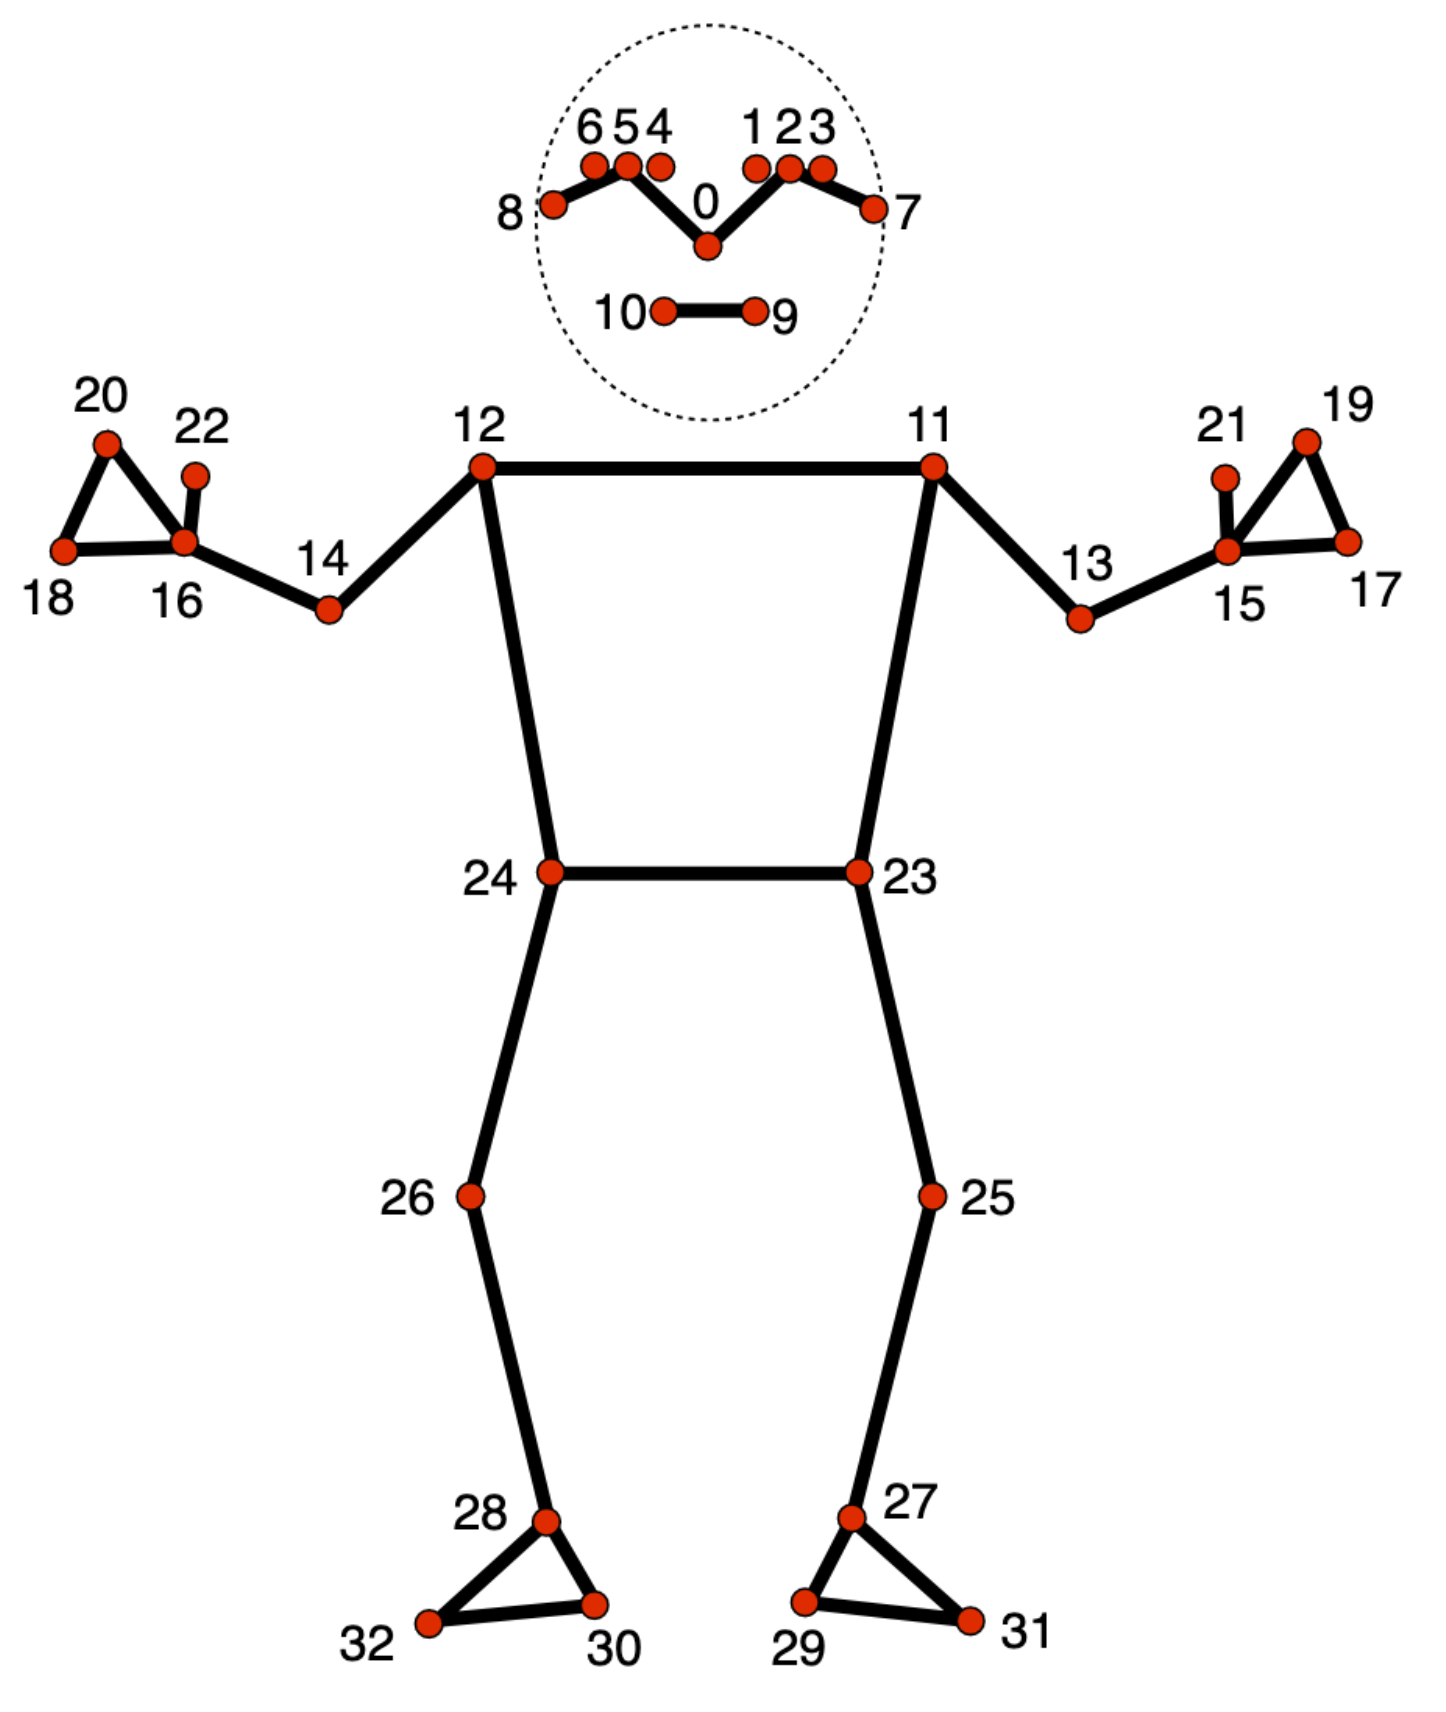
\includegraphics[height=0.8\textheight, keepaspectratio]{pose_landmarks_index.png}
        \vspace{0.2cm}
        {\small Keypoints cơ bản trong HPE (Human Pose Estimation).}
    \end{column}

    \begin{column}{0.55\textwidth}
        \begin{block}{Khái niệm}
            Ước lượng vị trí khớp từ hình ảnh/video:
            \[
                \mathcal{K} = \{k_i = (x_i, y_i, z_i, c_i)\}
            \]
            \small{\textit{($c_i$ là confidence score cho mỗi keypoint).}}
        \end{block}

        \begin{alertblock}{Phương pháp}
            \begin{itemize}
                \item \textbf{Top-down:} Phát hiện người trước, sau đó keypoints (MediaPipe).
                \item \textbf{Bottom-up:} Keypoints trước, nhóm thành người sau (OpenPose).
            \end{itemize}
        \end{alertblock}
    \end{column}
\end{columns}
\end{frame}

% Slide 3: MediaPipe Pose – Kiến trúc BlazePose
\begin{frame}{MediaPipe Pose – Kiến trúc BlazePose}
    \begin{block}{Kiến trúc BlazePose}
        BlazePose tối ưu HPE 3D với:
        \begin{itemize}
            \item \textbf{Nodes:} Các module xử lý tín hiệu hình ảnh.
            \item \textbf{Edges:} Luồng dữ liệu đồng bộ giữa các module.
        \end{itemize}
        \small{\textit{(Nodes = các bước tính toán; Edges = kết nối dữ liệu giữa các bước).}}
    \end{block}
\end{frame}

% Slide 4: MediaPipe Pose – Thành phần & Hậu xử lý
\begin{frame}{MediaPipe Pose – Thành phần & Hậu xử lý}
    \begin{exampleblock}{Thành phần chính}
        \begin{itemize}
            \item \textbf{Detection:} ROI từ ảnh RGB, phát hiện người.
            \item \textbf{Landmark:} 33 keypoints 3D, Loss: $\mathcal{L} = \sum \lambda_i \mathcal{L}_i$.
            \item \textbf{Tracking:} Dự đoán vị trí ROI cho khung tiếp theo.
        \end{itemize}
        \small{\textit{(Landmark 3D giúp đánh giá tư thế và động tác).}}
    \end{exampleblock}

    \begin{alertblock}{Hậu xử lý}
        \begin{itemize}
            \item \textbf{One Euro Filter:} Làm mịn nhiễu trong dữ liệu keypoints.
            \item \textbf{Chuẩn hóa $z$:} Dựa trên hông, tăng độ chính xác 3D.
        \end{itemize}
    \end{alertblock}
\end{frame}

% Slide 5: Thuật toán Phát hiện Té ngã
\begin{frame}{Thuật toán Phát hiện Té ngã}
    \begin{columns}[T]
        \column{0.5\textwidth}
        \begin{block}{Đặc trưng Động học}
            \begin{itemize}
                \item \textbf{Vận tốc COM:} $\vec{v}_{\text{COM}} = \frac{\Delta \vec{p}}{\Delta t}$
                \item \textbf{Gia tốc:} $a = \frac{\|\Delta \vec{v}\|}{\Delta t}$
            \end{itemize}
        \end{block}
        \begin{block}{Đặc trưng Tư thế}
            \begin{itemize}
                \item \textbf{AR (Aspect Ratio):} Tăng khi người nằm ngang
                \item \textbf{$\theta_{\text{body}}$:} Góc vai-hông
                \item \textbf{$\Delta h_{\text{head}}$:} Giảm chiều cao đầu
            \end{itemize}
            \small{\textit{(AR, $\theta$, $\Delta h$ giúp xác định tư thế bất thường).}}
        \end{block}

        \column{0.5\textwidth}
        \begin{alertblock}{Ba Giai đoạn Phát hiện}
            \begin{enumerate}
                \item \textbf{Sớm:} Tốc độ/gia tốc COM cao
                \item \textbf{Xác nhận:} AR, $\theta_{\text{body}}$ chỉ nằm ngang
                \item \textbf{Bất động:} Chuyển động $< M_{th}$
            \end{enumerate}
        \end{alertblock}
    \end{columns}
\end{frame}

% Slide 5: Thuật toán Phát hiện Té ngã
\begin{frame}{Thuật toán Phát hiện Té ngã}
    \begin{columns}[T]
        \column{0.5\textwidth}
        \begin{block}{Đặc trưng Động học}
            \begin{itemize}
                \item \textbf{Vận tốc COM:} $\vec{v}_{\text{COM}} = \frac{\Delta \vec{p}}{\Delta t}$
                \item \textbf{Gia tốc:} $a = \frac{\|\Delta \vec{v}\|}{\Delta t}$
            \end{itemize}
        \end{block}
        \begin{block}{Đặc trưng Tư thế}
            \begin{itemize}
                \item \textbf{AR (Aspect Ratio):} Tăng khi người nằm ngang
                \item \textbf{$\theta_{\text{body}}$:} Góc vai-hông
                \item \textbf{$\Delta h_{\text{head}}$:} Giảm chiều cao đầu
            \end{itemize}
            \small{\textit{(AR, $\theta$, $\Delta h$ giúp xác định tư thế bất thường).}}
        \end{block}

        \column{0.5\textwidth}
        \begin{alertblock}{Ba Giai đoạn Phát hiện}
            \begin{enumerate}
                \item \textbf{Sớm:} Tốc độ/gia tốc COM cao
                \item \textbf{Xác nhận:} AR, $\theta_{\text{body}}$ chỉ nằm ngang
                \item \textbf{Bất động:} Chuyển động $< M_{th}$
            \end{enumerate}
        \end{alertblock}
    \end{columns}
\end{frame}

